\problemname{Pickle clicker}
About half a year ago, the hit game Pickle Clicker was released. Rasmus has decided to take things
to the next level: he plans to speedrun the game. The in-game currency is, of course, pickles. The goal
is to buy the megapickle as quickly as possible, which costs $t$ pickles. There are $n$ types of buildings
in the game, each producing $p_i$ pickles per second and costing $c_i$ pickles. At the beginning, you own
one building of type 1. Every second, each building you own produces $p_i$ pickles. You then have the
alternative to build a building which you can afford. If you choose to build a building of type $i$,
you will pay $c_i$ pickles, but start making $p_i$ more pickles each following round.
While you can only build one building per turn, you can have multiple buildings of the same type
throughout the game.

Help Rasmus determine how to play the game so that he can buy the megapickle in as few seconds as possible.

\section*{Input}
The first line of input contains the integer $n$ ($1 \le n \le 6$), the number of types of buildings.

The following $n$ lines contain the integers $p_i, c_i$ ($1 \leq p_i, c_i \leq 10^5$), indicating how many pickles each building of type $i$ produces per second and its cost.

Finally, a line with the integer $t$ ($1 \le t \le 10^5$) follows, representing the cost of the megapickle.

\section*{Output}
Print an integer: the number of seconds it takes to afford the megapickle by playing optimally.

\section*{Points}
Your solution will be tested on several test case groups.
To get the points for a group, it must pass all the test cases in the group.

\noindent
\begin{tabular}{| l | l | p{12cm} |}
  \hline
  \textbf{Group} & \textbf{Point value} & \textbf{Constraints} \\ \hline
  $1$    & $20$       & $n=1$ \\ \hline
  $2$    & $20$       & $t \leq 10$ \\ \hline
  $3$    & $20$       & $t \leq 1000$ \\ \hline
  $4$    & $40$       & No additional constraints. \\ \hline
\end{tabular}

\section*{Sample explanation}

\begin{figure}[h]
  \centering
  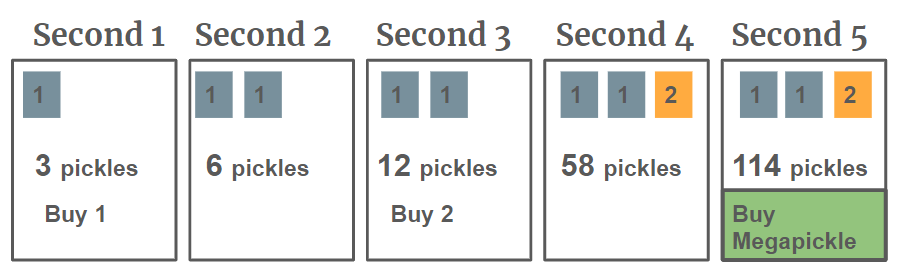
\includegraphics[width=0.7\textwidth]{sample1-en.PNG}
    \\The image shows the solution to sample 1. The first row describes which buildings 
    we own at the start of the corresponding second. The second row is how many pickles 
    we have after the buildings have produced. The last row indicates whether we bought
    something at the end of the second.
  
\end{figure}
